\section{Botnets}
\label{sec:botnets}

A \textit{botnet} is a network made up of unaware remote-controlled computers, typically used for malicious purposes.
A \textit{bot} is the malware that makes the infected host remotely controllable by a server - namely a \textit{controller} -  instructed by an attacker. Once started, the bot contacts the controller to join the \textit{botnet} and polls it for commands to execute.

Some botnets consist of hundreds of thousands — or even millions — of computers. Since they allow hundreds of thousands of different computers to act in unison, a botnet could be used to perform distributed DDoS attacks, massive spam campaign, click frauds, Bitcoin mining, or used to distribute other malwares, such as keyloggers, crypto lockers and so on. From this brief description it is possible to guess the economic implications of such a tool. \Cref{fig:botnet-showcase} depicts a simple but common botnet-based application.

A \textit{controller} - also known as \textit{command\&control server} - is a server that provides commands for bots to poll through interfaces - e.g. REST interfaces - hidden by a legitimate appearance - e.g. a showcase website.

\begin{figure}[tp]
  \centering
  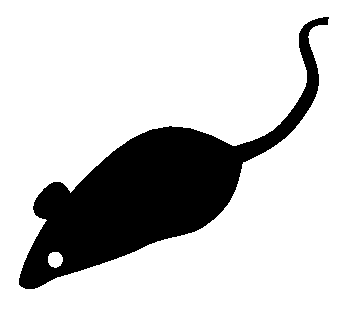
\includegraphics{./fig/acmlarge-mouse}
  \caption{A botnet showcase. (1) The attacker spreads bots via an infection vector - e.g. a trojan horse. (2) The infected hosts join the botnet, being remotely controllable by the attacker, via a command\&control server. (3) The computational power of the botnet is rent, for wichever malicious purpose, making the attacker gaining a lot of profits. (4) The attacker instructs the botnet to perform a spamming campaign, as requested by its client.}
    \label{fig:botnet-showcase}
\end{figure}

Botnets can be controlled in several different ways, depending on how the command\&control layer is implemented.

In its simplest form, it implements a centralized client-server architecture, where bots poll a web server for commands to execute. Such a botnet is easy to stop — monitor what web servers a bot is connecting to, then go and take down those web servers. The bots will be unable to communicate with their creators.

In a more advanced form, it implements a peer-to-peer architecture, where bots instruct (are instructed by) other nearby bots, thus providing the botnet with a high degree of availability and redundancy. Since no single point of control can be identified, such botnets cannot be neutered only by disabling specific nodes. Therefore, defensive strategies are based on issuing fake commands or by isolating the bots from each other.

Things are made harder since botnets started communicating, not only through encrypted channels, but via the Tor network, where it’s theoretically impossible to figure out the botnet topology.

Symantec’s study of the ZeroAccess botnet shows us an example. The ZeroAccess botnet is one of the largest known botnetswith a population upwards of 1.9 million computers, generating profits through Bitcoin mining and click fraud. \cite{zeroaccess-symantec-blog,zeroaccess-symantec-definition}.
A key feature of the ZeroAccess botnet is its use of a peer-to-peer (P2P) command-and-control (C\&C) communications architecture, with a constant communication between peers. Each peer continuously connects with other peers to exchange peer lists and check for updated files, making it highly resistant to any take-down attempts.
